\documentclass[border=10pt]{standalone}
\usepackage{xcolor}
\usepackage{tikz}
\usetikzlibrary{arrows.meta,fit,backgrounds,positioning}

\definecolor{INK}{HTML}{1A1A2E}
\definecolor{BG}{HTML}{FAFAFA}
\definecolor{SUB}{HTML}{555566}
\definecolor{COLD}{HTML}{4361EE}
\definecolor{WARM}{HTML}{2EC4B6}
\definecolor{NEW}{HTML}{F4A261}
\definecolor{JOB}{HTML}{D81159}

\begin{document}
\pagecolor{BG}
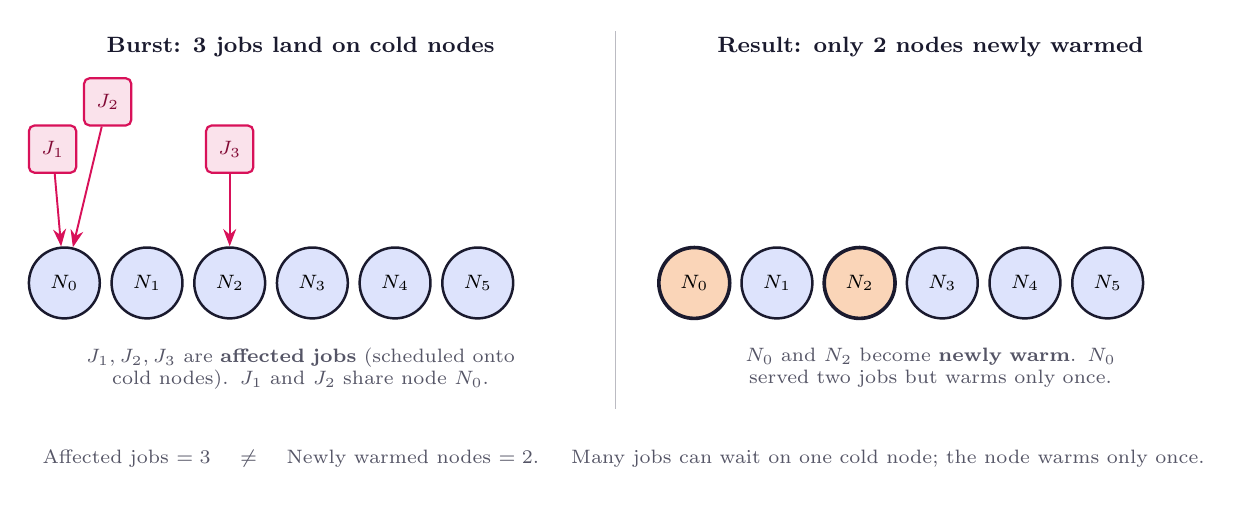
\begin{tikzpicture}[
    font=\sffamily,
    nd/.style={circle, draw=INK, line width=0.9pt, minimum size=9mm, inner sep=0pt, font=\scriptsize\bfseries},
    cold/.style={nd, fill=COLD!18},
    warm/.style={nd, fill=WARM!22},
    newwarm/.style={nd, fill=NEW!45, line width=1.3pt},
    job/.style={draw=JOB, fill=JOB!12, line width=0.8pt, rounded corners=2pt, minimum size=6mm, inner sep=1pt, font=\scriptsize\bfseries, text=JOB!60!black},
    arr/.style={-{Stealth[length=2.2mm]}, JOB, line width=0.7pt},
    head/.style={font=\footnotesize\bfseries, text=INK},
    sub/.style={font=\scriptsize, text=SUB},
  ]

  % ===== LEFT: burst assignment =====
  \begin{scope}[xshift=0cm]
    \node[head] at (3.0, 3.0) {Burst: 3 jobs land on cold nodes};
    % nodes
    \foreach \i/\sty in {0/cold,1/cold,2/cold,3/cold,4/cold,5/cold} {
      \node[\sty] (a\i) at (\i*1.05, 0) {$N_\i$};
    }
    % jobs
    \node[job] (j1) at (-0.15, 1.7) {$J_1$};
    \node[job] (j2) at (0.55, 2.3) {$J_2$};
    \node[job] (j3) at (2.1, 1.7) {$J_3$};
    \draw[arr] (j1) -- (a0);
    \draw[arr] (j2) -- (a0);
    \draw[arr] (j3) -- (a2);
    \node[sub, anchor=north, text width=6.2cm, align=center] at (3.0, -0.7)
      {$J_1, J_2, J_3$ are \textbf{affected jobs} (scheduled onto cold nodes). $J_1$ and $J_2$ share node $N_0$.};
  \end{scope}

  % divider
  \draw[SUB!40, line width=0.6pt] (7.0, -1.6) -- (7.0, 3.2);

  % ===== RIGHT: newly warmed result =====
  \begin{scope}[xshift=8.0cm]
    \node[head] at (3.0, 3.0) {Result: only 2 nodes newly warmed};
    \node[newwarm] (b0) at (0*1.05, 0) {$N_0$};
    \node[cold]    (b1) at (1*1.05, 0) {$N_1$};
    \node[newwarm] (b2) at (2*1.05, 0) {$N_2$};
    \node[cold]    (b3) at (3*1.05, 0) {$N_3$};
    \node[cold]    (b4) at (4*1.05, 0) {$N_4$};
    \node[cold]    (b5) at (5*1.05, 0) {$N_5$};
    \node[sub, anchor=north, text width=6.2cm, align=center] at (3.0, -0.7)
      {$N_0$ and $N_2$ become \textbf{newly warm}. $N_0$ served two jobs but warms only once.};
  \end{scope}

  % ===== bottom key formula =====
  \node[sub, anchor=north west] at (-0.4, -2.0)
    {Affected jobs $=3$ \quad $\neq$ \quad Newly warmed nodes $=2$. \quad Many jobs can wait on one cold node; the node warms only once.};

\end{tikzpicture}
\end{document}
